\rulesection{2.0 Components}

\textit{Shenandoah: Valley of Fire} includes these rules, one 22" by 34" map, a scenario record chart for each player, a holding box and chart card, and a set of 200 die-cut counters. If any component is defective, please return it for prompt replacement. You will also need two six-sided dice.

\rulesubsection{2.1 Map}

The map is divided into hexagons, called hexes, that define the units' positions like squares on a chessboard. The map depicts the area where the campaigns occurred.

\textbf{2.11 River and Stream Hexes.} The map includes two kinds of waterways: rivers and streams. Effects described for rivers do not apply to streams.

\rulesubsection{2.2 Counters}

\textbf{2.21 Leaders.} A leader is a counter with an infantry, cavalry, or artillery symbol. A leader represents that commander with his accompanying troops. Each leader has a troop strength, made up of strength points (SPs) and recorded on the Player Record Sheet. SPs may be transferred from one leader to another only through detachment and reattachment. A leader can control only the troop type indicated by his symbol. If a unit loses all its SPs, remove it from play.

\textbf{2.22 Commanders.} A commander is a counter with a name and one or more stars. It represents a high-ranking officer with no accompanying troops. Commanders include one supreme commander for each side, plus one cavalry commander for each side. In the 1862 scenarios the Union has more than one supreme commander. When a rule applies to both commanders and leaders, commanders will be called leaders as well. SPs may not be attached to commanders.

\begin{center}
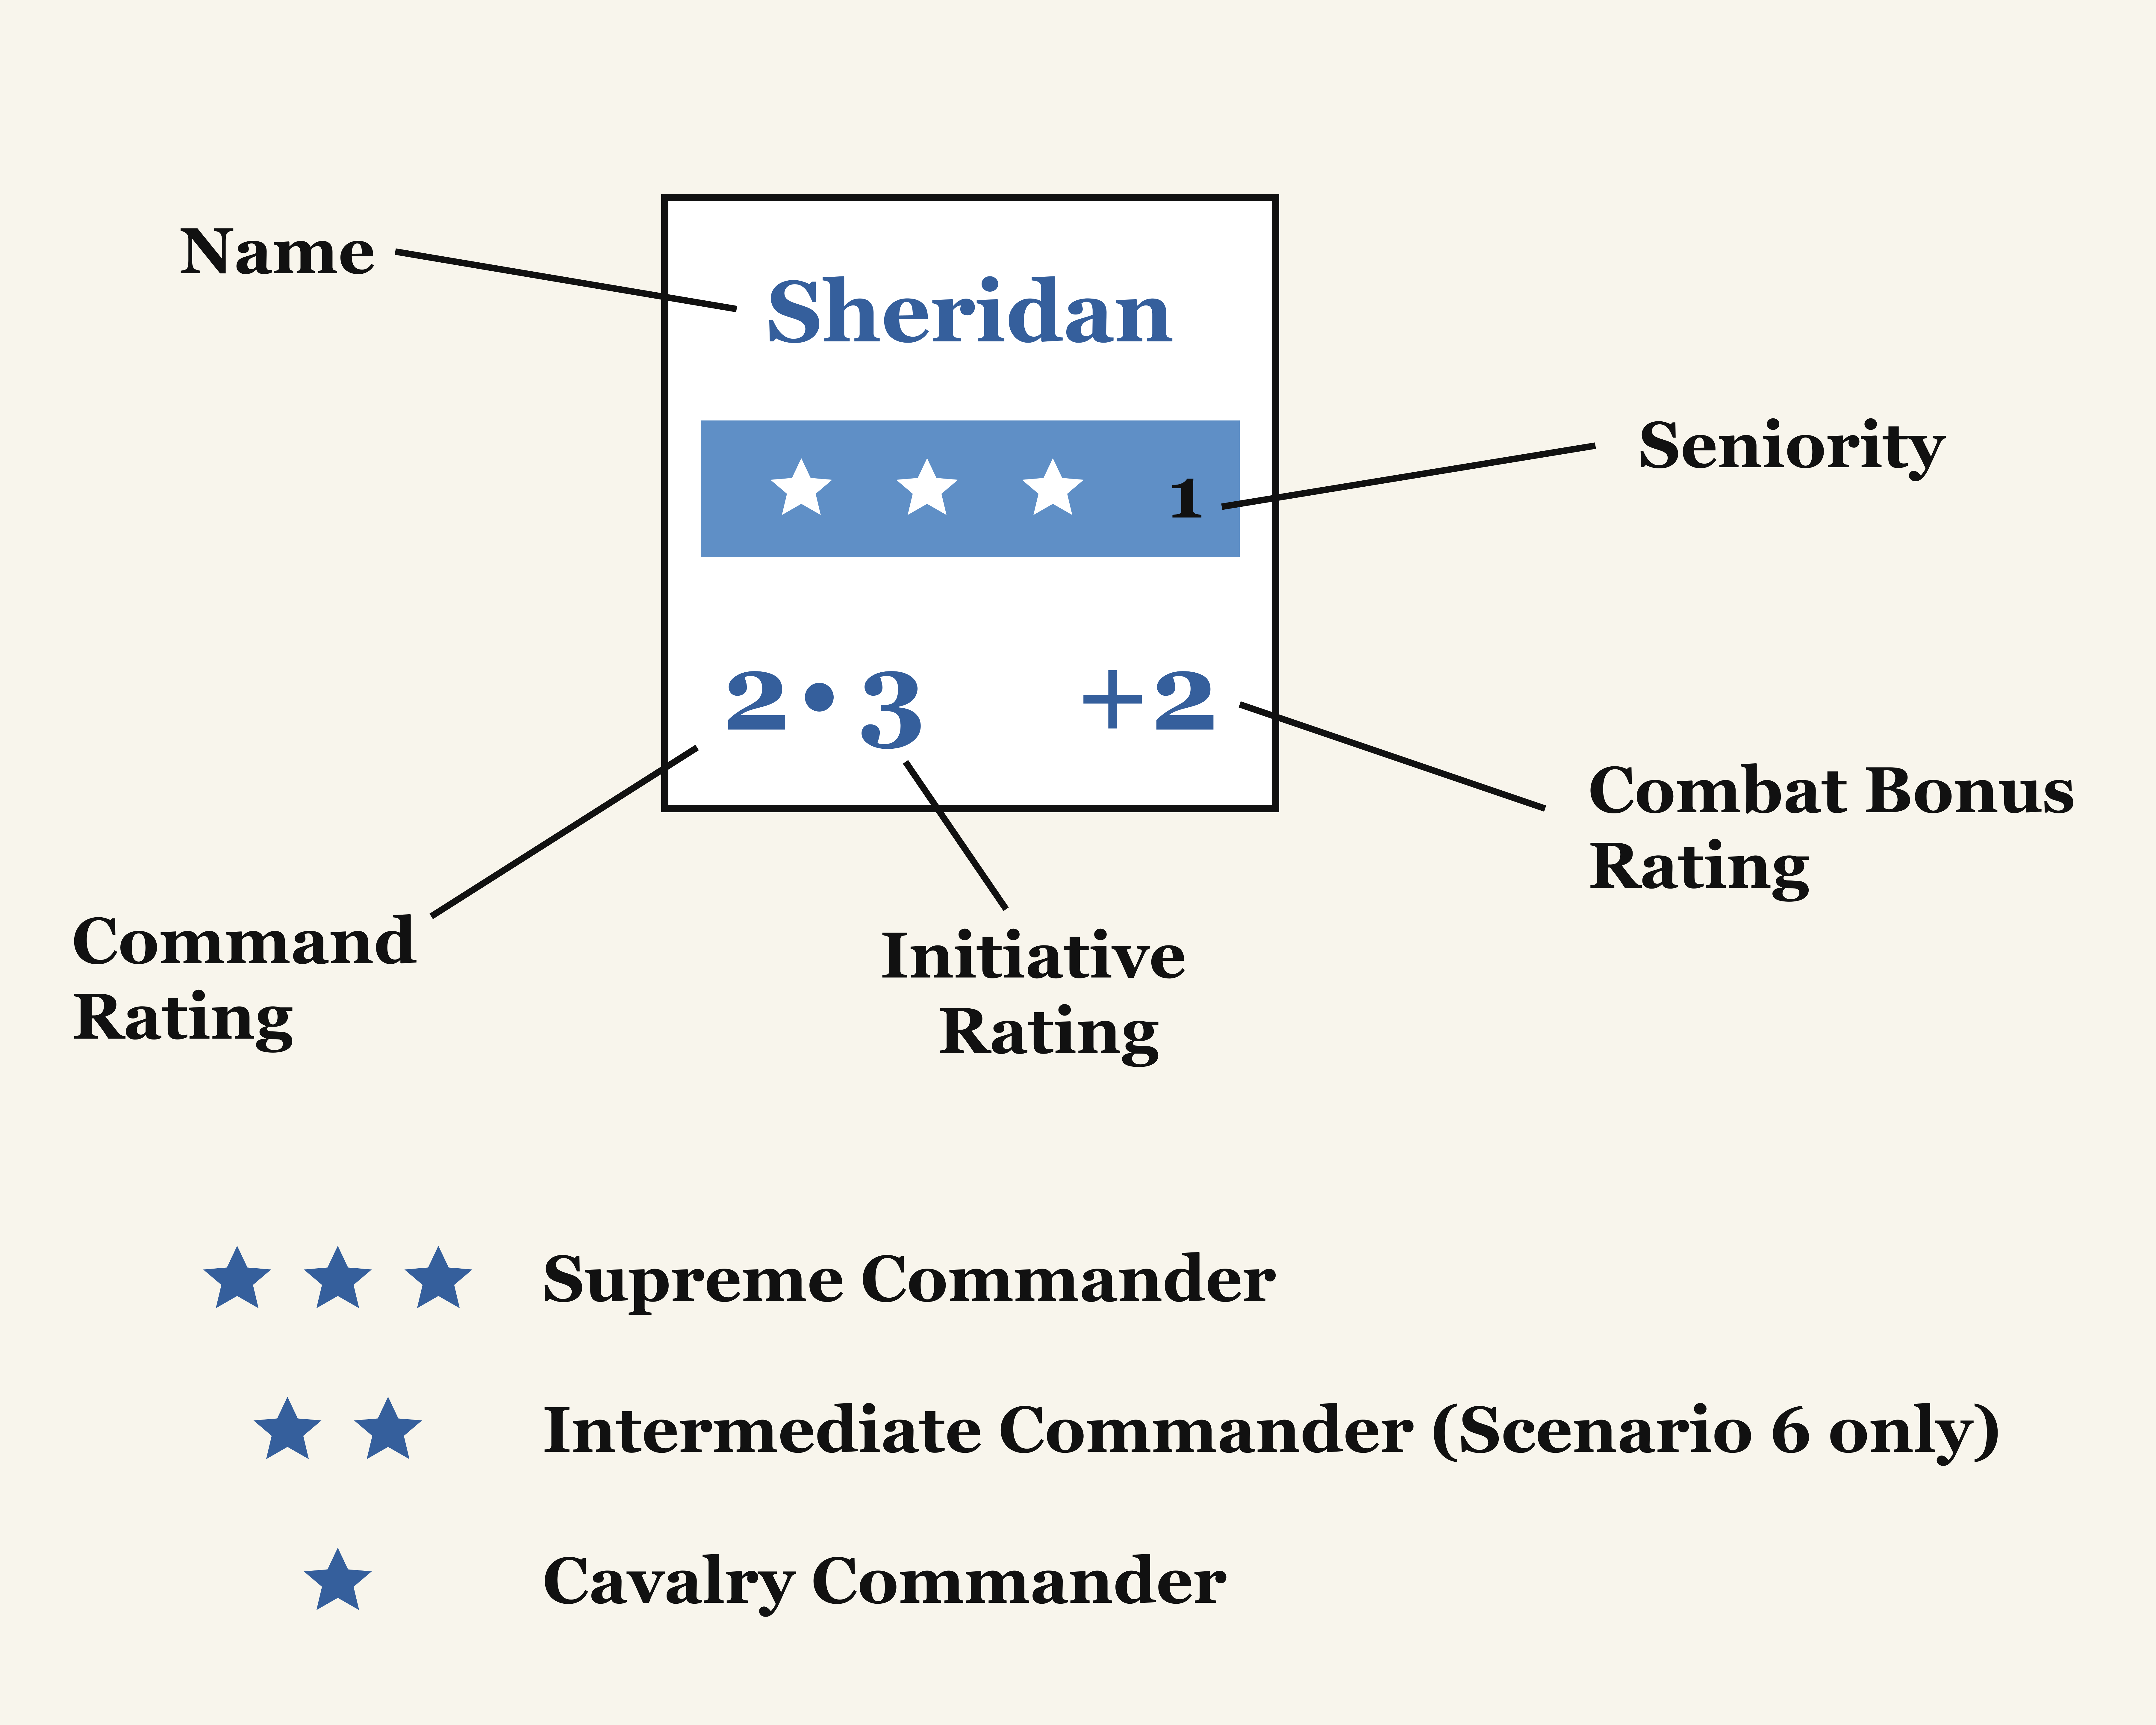
\includegraphics[width=0.86\columnwidth]{Images/sample_commander_counter.png}

\vspace{0.6em}

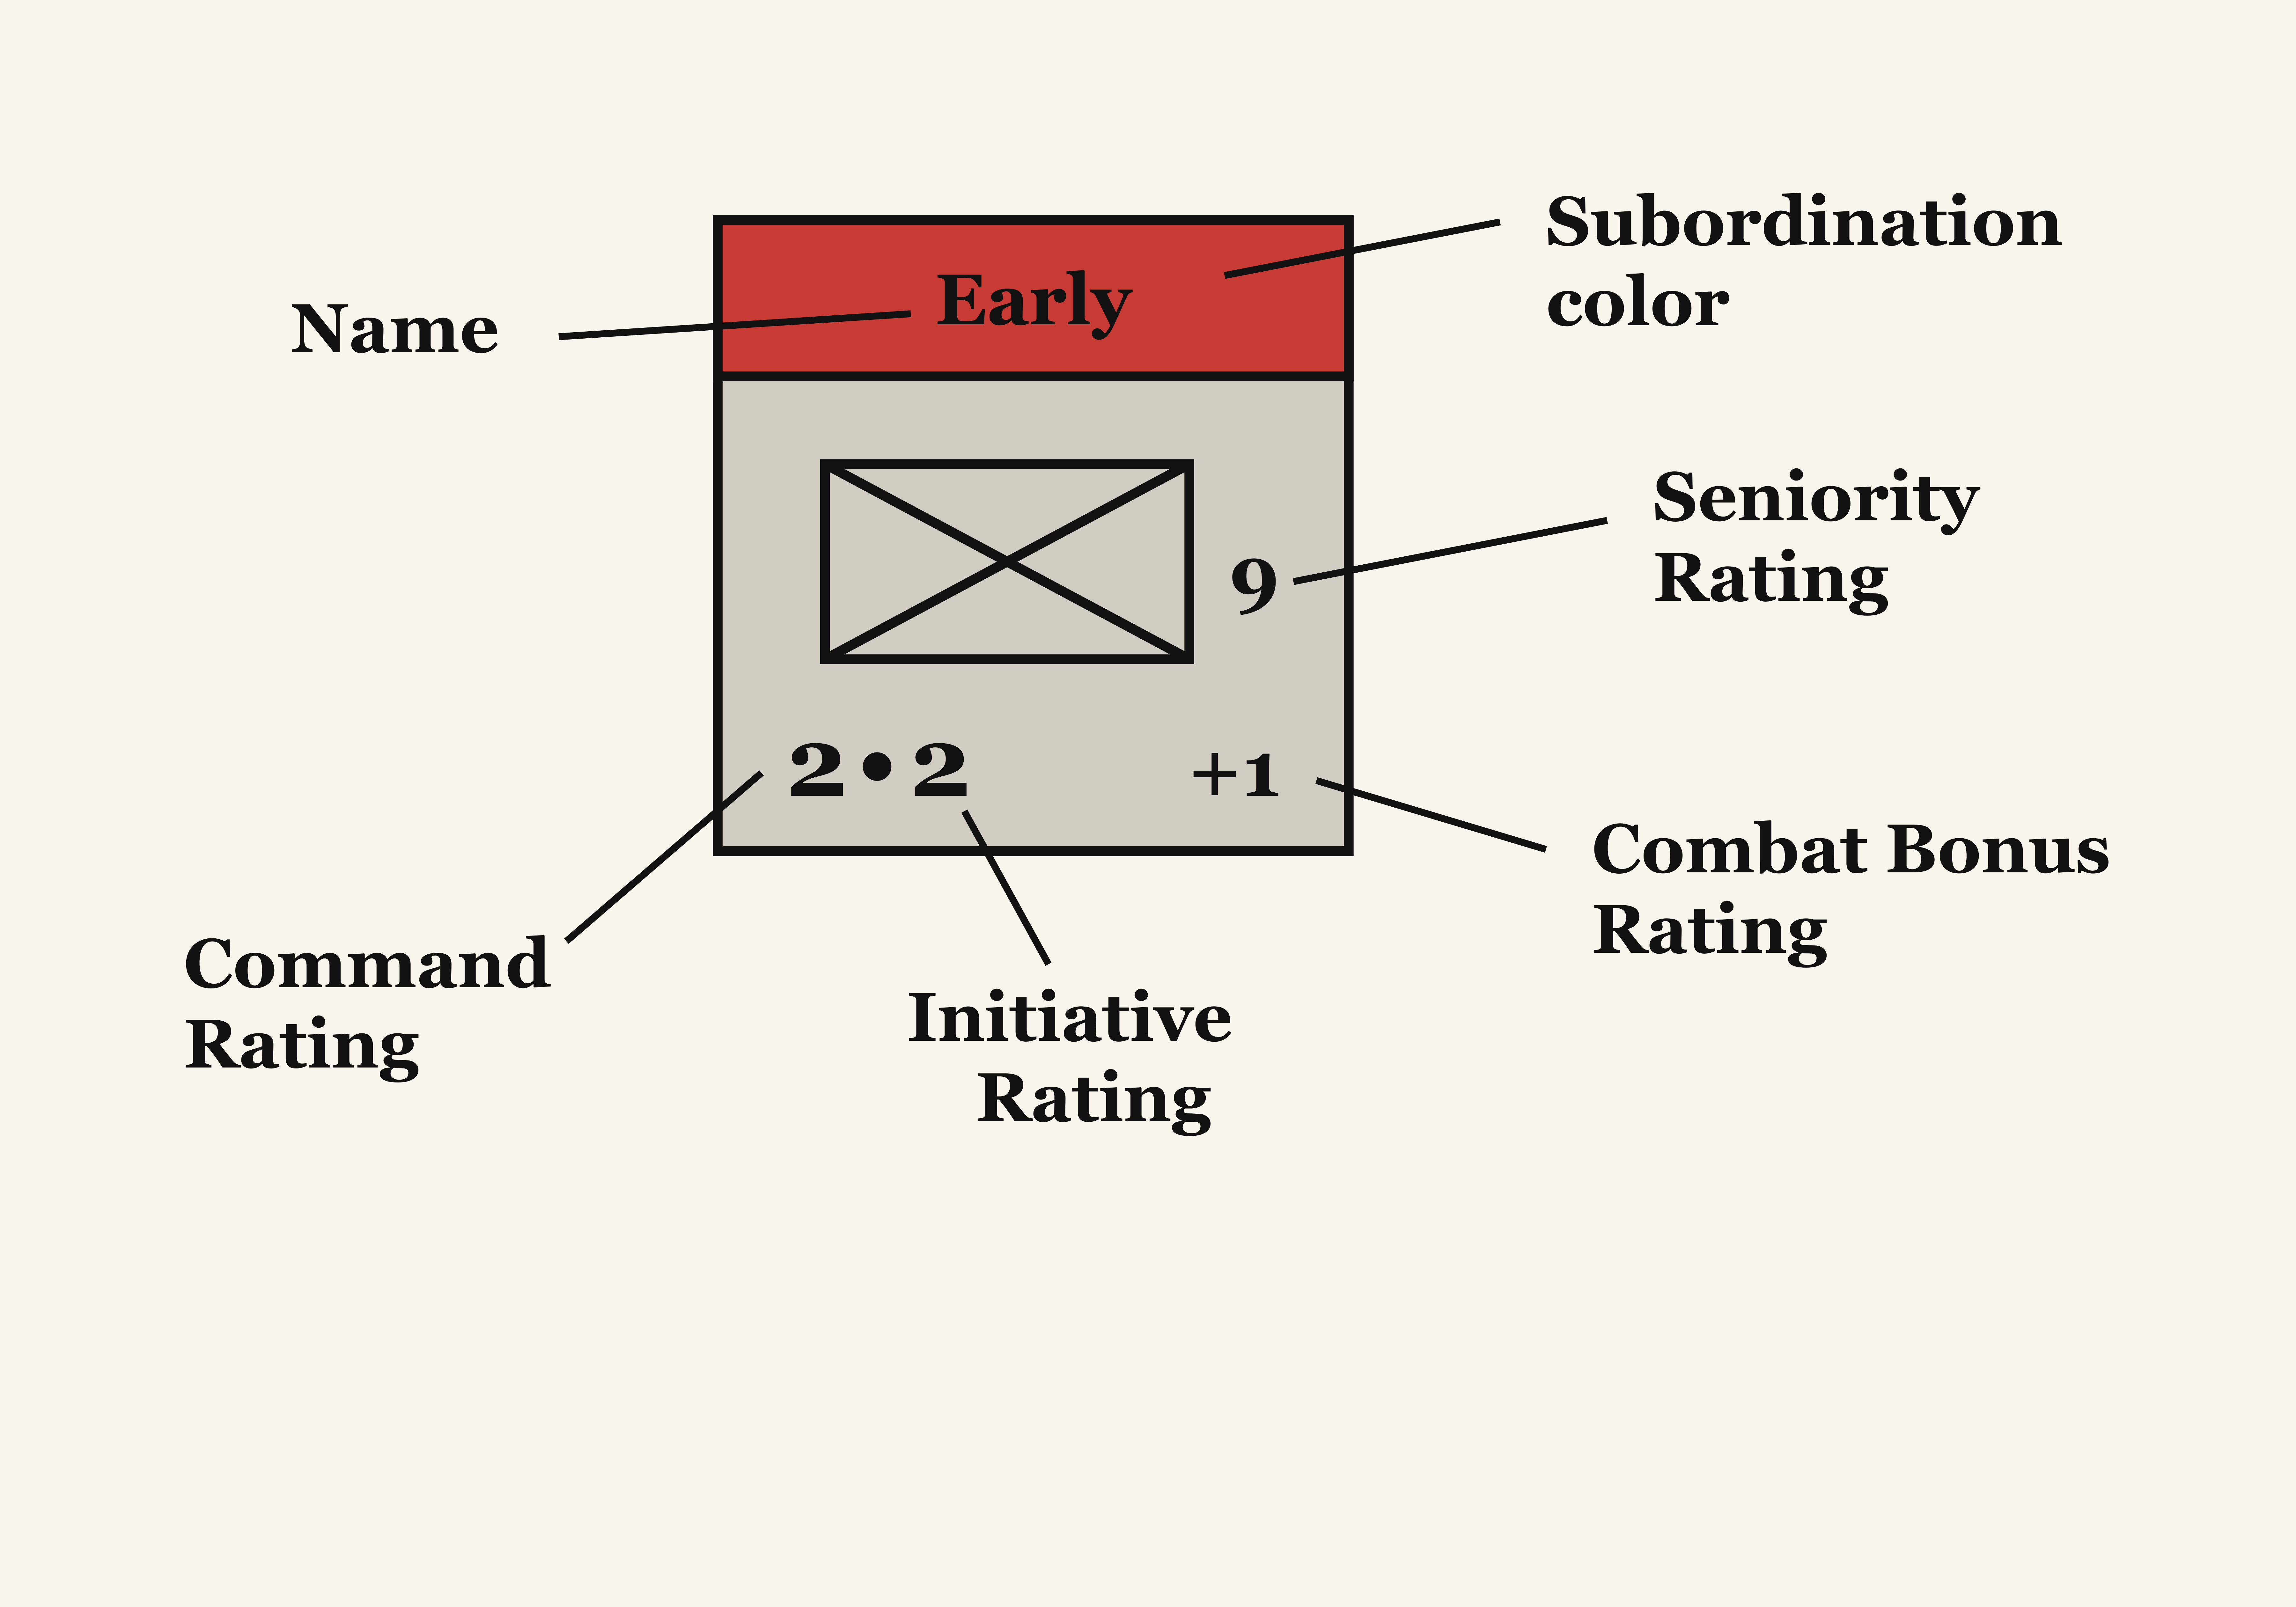
\includegraphics[width=0.86\columnwidth]{Images/sample_combat_unit_counter.png}
\end{center}

\textbf{2.23 Unit Sizes.} Each infantry and cavalry unit, except detachments, represents a division. A detachment has no formal size, but is smaller than a division.

\textbf{2.25 Marker Summary.} Markers include rail cut, constructing entrenchment, entrenchment, panic, command points received, bridge destroyed, entrained, and devastation.

\rulesubsection{2.3 Game Scale}

Each hex is approximately two miles across. Each SP represents 300 men. Each turn represents two days.

\rulesubsection{2.4 Charts and Tables}

These are used to determine movement allowances and costs, and to resolve combat.

\textbf{2.41 Holding Boxes.} Often many pieces will be stacked together with a high-ranking leader such as Sheridan or Jackson. When this occurs, players may place all lower-ranking units in the holding box where the leader's name appears on the chart card. Units in a holding box are considered to occupy the same hex as the corresponding leader; units may be moved between the holding box and map at any time. The holding boxes are purely for convenience.

\rulesubsection{2.5 Percentage Chart}

Game procedures will require players to compute percentages of a unit's strength or movement allowance. Locate the row corresponding to the original value and cross-reference it with the needed percentage column. If the exact original value is not listed, choose two row numbers that total the original value, find the percentages separately, and add the results.

\textbf{Example.} To find 50\% of a force whose original size is 27, use 25 plus 2. The chart gives 13 for the 25 row and 1 for the 2 row; together this yields 14.

\rulesubsection{2.6 Player Record Sheets}

Each player has a separate Player Record Sheet for the scenarios. The record sheet shows when and where each leader enters play. Players also use the sheet to record the current strengths of combat units. These should be photocopied before use. Each player's record sheet is kept secret from the opponent.

\rulesubsection{2.7 Die Roll Modifiers}

Many events in the game require one or two dice. Certain conditions add to or subtract from the result. These are called die roll modifiers, abbreviated DRMs.
